\section{Auswertung}\label{sec:auswertung}
\newcommand{\tikztextc}[3]{\node at (#1, #2) {\vphantom{/}\smash{#3}};}
\newcommand{\tikztextupc}[3]{\node at (#1, #2) [rotate = 90] {\vphantom{/}\smash{#3}};}
\definecolor{myRed}{RGB}{255, 119, 94}
\definecolor{myGreen}{RGB}{140, 255, 144}
Zur Auswertung, wie gut ein Analyseverfahren abgeschnitten hat, wurden zwei Klassifizierungen vorgenommen. Einmal wurden die tatsächlichen Ausreißer und Nachbarn markiert -- also die, die auf den originalen Zeitreihen erkannt wurden -- und einmal wurden die vorhergesagten Ausreißer und Nachbarn markiert -- also die, die auf den komprimierten Zeitreihen erkannt wurden. Nachdem alle Zeitreihen klassifiziert waren, konnte eine sogenannte Konfusionsmatrix erstellt werden, die Grundlage für häufig genutzte Metriken ist \cite{konfusionsmatrix}. \autoref{fig:konfusionsmatrix} zeigt wie eine solche Konfusionsmatrix aussieht. Die Klassifizierungen führen zu vier Fällen: \begin{enumerate}
    \item die Anzahl der Zeitreihen, die in den originalen und komprimierten Zeitreihen markiert wurden, zählen zu richtig positiv (engl. \textit{\textbf{T}rue \textbf{P}ositive}),
    \item die Anzahl der Zeitreihen, die nicht in den originalen aber in den komprimierten Zeitreihen markiert wurden, zählen zu falsch positiv (engl. \textit{\textbf{F}alse \textbf{P}ositive}),
    \item die Anzahl der Zeitreihen, die nicht in den originalen und nicht in den komprimierten Zeitreihen markiert wurden, zählen zu richtig negativ (engl. \textit{\textbf{T}rue \textbf{N}egative}),
    \item die Anzahl der Zeitreihen, die in den originalen aber nicht in den komprimierten Zeitreihen markiert wurden, zählen zu falsch negativ (engl. \textit{\textbf{F}alse \textbf{N}egative}).
\end{enumerate} 

Aus diesen vier Werten können nun mehrere Metriken berechnet werden, wobei für uns nur Präzision (engl. \textit{\textbf{Prec}ision}), Sensitivität (engl. \textit{\textbf{Rec}all}) und das $\text{F}_1$"=Maß (engl. \textit{F$_1$"=Score}) von Bedeutung sind.

Die Präzision berechnet sich mit der Formel: \[Prec = \frac{TP}{TP + FP}\]
und beschreibt in unserem Fall, wie viele der als Ausreißer / Nachbar erkannten Punkte tatsächlich Ausreißer / Nachbar sind.

Die Sensitivität berechnet sich mit der Formel \[Rec = \frac{TP}{TP + FN}\] und beschreibt in unserem Fall, wie viele der tatsächlichen Ausreißer / Nachbar erkannt wurden.

Das F$_1$"=Maß ist das harmonische Mittel der zwei vorherigen Werte. Es berechnet sich wie folgt: \[\text{F}_1=2\cdot\frac{Prec \cdot Rec}{Prec + Rec}\] und ermöglicht es zu bewerten, wie zuverlässig ein Verfahren ist, da es Sensitivität und Präzision kombiniert. Nur wenn beide Werte hoch sind, also wenn wenige bis keine falschen Entscheidungen getroffen wurden (Präzision) und nahezu alle ursprünglichen Ausreißer / Nachbarn gefunden wurden (Sensitivität), nur dann ist auch das F$_1$"=Maß hoch. Beispielsweise ist das harmonische Mittel der Zahlen 0,1 und 0,9 gleich 0,18, das
heißt der kleinere (schlechtere) Wert dominiert das Ergebnis.
\begin{figure}[h]
\centering
 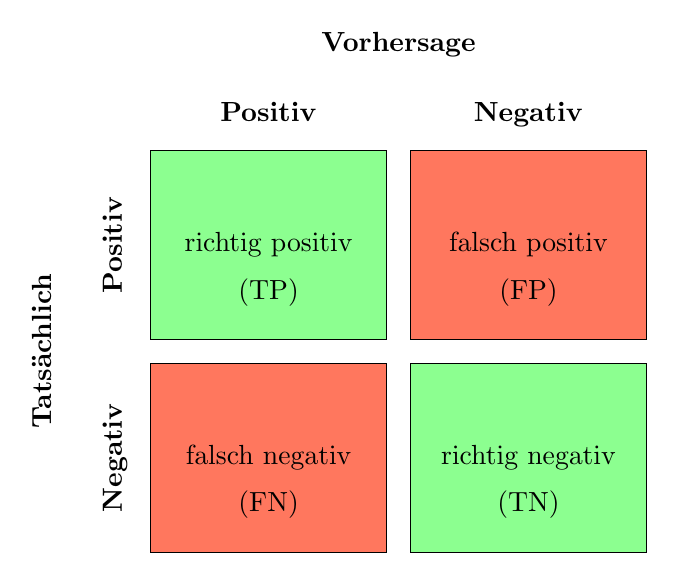
\begin{tikzpicture}[x = 3mm, y = 3mm]   % das hier verändern zum Skalieren
    % Bounding box
  \useasboundingbox (-5.2, -0.1) rectangle (21.2, 22.2);
  % links unten
  \filldraw [draw = black, fill = myRed] (0, 0) rectangle ++(10, 8);
  \tikztextc{5}{4}{falsch negativ}
  \tikztextc{5}{2}{(FN)}
  % rechts unten
  \filldraw [draw = black, fill = myGreen] (11, 0) rectangle ++(10, 8);
  \tikztextc{16}{4}{richtig negativ}
  \tikztextc{16}{2}{(TN)}
  % links oben
  \filldraw [draw = black, fill = myGreen!] (0, 9) rectangle ++(10, 8);
  \tikztextc{5}{13}{richtig positiv}
  \tikztextc{5}{11}{(TP)}
  % rechts oben
  \filldraw [draw = black, fill = myRed] (11, 9) rectangle ++(10, 8);
  \tikztextc{16}{13}{falsch positiv}
  \tikztextc{16}{11}{(FP)}
  % daneben
  \tikztextupc{-1.5}{4}{\textbf{Negativ}}
  \tikztextupc{-1.5}{13}{\textbf{Positiv}}
  \tikztextupc{-4.5}{8.5}{\textbf{Tatsächlich}}
  % drüber
  \tikztextc{5}{18.5}{\textbf{Positiv}}
  \tikztextc{16}{18.5}{\textbf{Negativ}}
  \tikztextc{10.5}{21.5}{\textbf{Vorhersage}}
 \end{tikzpicture}
 \caption{Konfusionsmatrix}
 \label{fig:konfusionsmatrix}
\end{figure}